% Ensure that you compile using XeLaTeX !!! PDFTex has problems with some of the packages used
\documentclass[12pt]{article}
\setlength\parindent{0pt}

\usepackage{parskip}
\usepackage[margin=0.5in]{geometry}
\usepackage{fullpage}
\usepackage{moresize}
\usepackage{graphicx}
\usepackage{caption}
\usepackage{subcaption}
\usepackage{float}
\usepackage{xcolor}
\usepackage{soul}
\usepackage{fontspec}
\setmainfont{Doulos SIL}

\begin{document}

\begin{center}
\textbf{{\color{violet}{\HUGE 20201013 Tuesday\\}}}

\textbf{{\color{violet}{\HUGE ALL EXAMS (with notes)\\}}}

\end{center}
\newpage

\begin{center}
\textbf{{\color{blue}{\HUGE START OF EXAM\\}}}

\textbf{{\color{blue}{\HUGE Student ID: empty\\}}}

\textbf{{\color{blue}{\HUGE 9:00\\}}}

\end{center}
\newpage

\begin{center}
\textbf{{\color{blue}{\HUGE START OF EXAM\\}}}

\textbf{{\color{blue}{\HUGE Student ID: 48772\\}}}

\textbf{{\color{blue}{\HUGE 9:10\\}}}

\end{center}
\newpage

{\large Question 1}\\

Topic: Skewed Distributions\\
Source: Week 5 Handout, Question 5\\

How would you look for co-occurrence restrictions between [s] and the vowels that come after it in this dataset?\\

\begin{figure}[H]
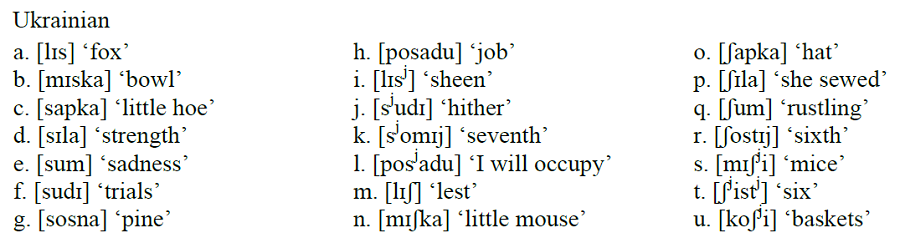
\includegraphics{../images/ukrainian.png}
\end{figure}

~\\
INSTRUCTOR NOTES: 


\vfill
Excellent (3) ~~~ Good (2.2) ~~~ Fair (1.7) ~~~ Poor (0)
\newpage

{\large Question 2}\\

Topic: Transcription\\
Source: Week 2 Handout, Part II\\

Is this a reasonable transcription of this word? Explain why.\\

<paid>: {[peid]}


~\\
INSTRUCTOR NOTES: okay, but [eɪ]


\vfill
Excellent (3) ~~~ Good (2.2) ~~~ Fair (1.7) ~~~ Poor (0)
\newpage

\begin{center}
\textbf{{\color{red}{\HUGE END OF EXAM}}}\\

\end{center}
\newpage

\begin{center}
\textbf{{\color{blue}{\HUGE START OF EXAM\\}}}

\textbf{{\color{blue}{\HUGE Student ID: empty\\}}}

\textbf{{\color{blue}{\HUGE 9:20\\}}}

\end{center}
\newpage

\begin{center}
\textbf{{\color{blue}{\HUGE START OF EXAM\\}}}

\textbf{{\color{blue}{\HUGE Student ID: empty\\}}}

\textbf{{\color{blue}{\HUGE 9:30\\}}}

\end{center}
\newpage

\begin{center}
\textbf{{\color{blue}{\HUGE START OF EXAM\\}}}

\textbf{{\color{blue}{\HUGE Student ID: 83639\\}}}

\textbf{{\color{blue}{\HUGE 9:40\\}}}

\end{center}
\newpage

{\large Question 1}\\

Topic: Phonological Features\\
Source: Week 4 Discussion\\

Explain why phonological features are used instead of phonetic characteristics in analyzing datasets.\\


~\\
INSTRUCTOR NOTES: Phonological features help to capture phonological patterns, i.e., they group sounds together based on whether they do things like triggering a change or undergoing a change. Phonological features are sometimes language-specific. Phonetic characteristics are simply descriptions of the physical properties of the sounds; they are language-universal and independent of the patterns (though it turns out that many phonological patterns are based on phonetic characteristic groupings).


\vfill
Excellent (3) ~~~ Good (2.2) ~~~ Fair (1.7) ~~~ Poor (0)
\newpage

{\large Question 2}\\

Topic: Transcription\\
Source: Week 2 Handout, Part II, Question 11\\

How would this word be transcribed?\\ Kathleen will likely ask a follow-up question about why you used a particular symbol.\\

<little>


~\\
INSTRUCTOR NOTES: [lɪɾl̩]


\vfill
Excellent (3) ~~~ Good (2.2) ~~~ Fair (1.7) ~~~ Poor (0)
\newpage

\begin{center}
\textbf{{\color{red}{\HUGE END OF EXAM}}}\\

\end{center}
\newpage

\begin{center}
\textbf{{\color{blue}{\HUGE START OF EXAM\\}}}

\textbf{{\color{blue}{\HUGE Student ID: 74431\\}}}

\textbf{{\color{blue}{\HUGE 9:50\\}}}

\end{center}
\newpage

{\large Question 1}\\

Topic: Other (pre-midterm)\\
Source: Week 4 Handout, Part II, Question 3\\

Explain how you would figure out what the Luiseño form is for the morpheme whose meaning is given below. (To be clear: you do NOT need to give me the form itself -- just explain the process of figuring it out.)\\

‘make / cause’

\begin{figure}[H]
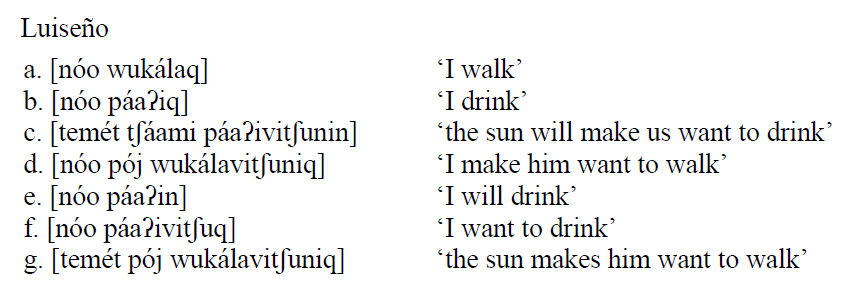
\includegraphics{../images/luiseno.png}
\end{figure}

~\\
INSTRUCTOR NOTES: ([ni])


\vfill
Excellent (3) ~~~ Good (2.2) ~~~ Fair (1.7) ~~~ Poor (0)
\newpage

{\large Question 2}\\

Topic: Skewed Distributions\\
Source: Week 5 Handout, Question 6\\

If I gave you a new word in Malto, [di\_\_u], would it be possible to predict whether it's [d] or [ɖ] that goes in the blank? Explain why or why not.\\


~\\
INSTRUCTOR NOTES: Yes, it's possible; in Malto, if there are two stops in a word, they must either both be dental or both retroflex. Since the first sound is dental, the second must also be dental (though to be fair, you couldn't actually predict that it's [d] and not [t], but the question restricts it to only the voiced options).


\vfill
Excellent (3) ~~~ Good (2.2) ~~~ Fair (1.7) ~~~ Poor (0)
\newpage

\begin{center}
\textbf{{\color{red}{\HUGE END OF EXAM}}}\\

\end{center}
\newpage

\begin{center}
\textbf{{\color{blue}{\HUGE START OF EXAM\\}}}

\textbf{{\color{blue}{\HUGE Student ID: 68935\\}}}

\textbf{{\color{blue}{\HUGE 4:00\\}}}

\end{center}
\newpage

{\large Question 1}\\

Topic: Phonological Features\\
Source: Week 4 Discussion\\

Explain what the given feature’s value is for this class of sounds, and why.\\

{[continuant]}

glottals


~\\
INSTRUCTOR NOTES: 0, because there is no constriction in the vocal tract for manner features to apply


\vfill
Excellent (3) ~~~ Good (2.2) ~~~ Fair (1.7) ~~~ Poor (0)
\newpage

{\large Question 2}\\

Topic: Articulatory Phonetics\\
Source: Week 3 Handout, Question 3\\

Explain why the additional vowel below either does or does not belong in the phonetic natural class defined by the original set of SNAE vowels.\\

Original set: {[æ]}, {[ɑ]}

Addition: {[ɑʊ]}


~\\
INSTRUCTOR NOTES: should recognize that there's more than one vowel sound, which makes it somewhat difficult to categorize; best answers will say that the diphthong is crucially a diphthong and so can't also go in this class


\vfill
Excellent (3) ~~~ Good (2.2) ~~~ Fair (1.7) ~~~ Poor (0)
\newpage

\begin{center}
\textbf{{\color{red}{\HUGE END OF EXAM}}}\\

\end{center}
\newpage

\begin{center}
\textbf{{\color{blue}{\HUGE START OF EXAM\\}}}

\textbf{{\color{blue}{\HUGE Student ID: 92054\\}}}

\textbf{{\color{blue}{\HUGE 4:10\\}}}

\end{center}
\newpage

{\large Question 1}\\

Topic: Phonological Features\\
Source: Quiz 3, Question 12\\

Explain how you figure out which feature is involved in the process of umlaut.\\

\begin{figure}[H]
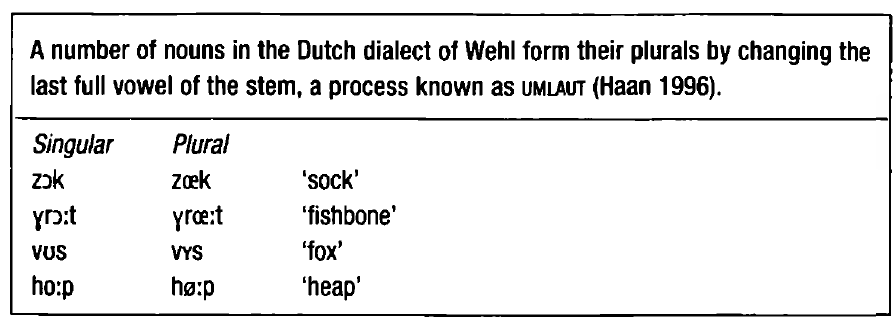
\includegraphics{../images/dutch.png}
\end{figure}

~\\
INSTRUCTOR NOTES: we look to see which vowels are affected, and compare them to see which feature is DIFFERENT (not e.g. what features they share); so since the vowels in the singular and plural are identical except that the singular forms are back and the plural are front, it's the feature [back] that is relevant / changing / involved (not e.g. the feature [round] just because all of the vowels are round)


\vfill
Excellent (3) ~~~ Good (2.2) ~~~ Fair (1.7) ~~~ Poor (0)
\newpage

{\large Question 2}\\

Topic: Transcription\\
Source: Week 2 Handout, Part II, Question 11\\

How would this word be transcribed?\\ Kathleen will likely ask a follow-up question about why you used a particular symbol.\\

<vacuum>


~\\
INSTRUCTOR NOTES: [vækjum]


\vfill
Excellent (3) ~~~ Good (2.2) ~~~ Fair (1.7) ~~~ Poor (0)
\newpage

\begin{center}
\textbf{{\color{red}{\HUGE END OF EXAM}}}\\

\end{center}
\newpage

\begin{center}
\textbf{{\color{blue}{\HUGE START OF EXAM\\}}}

\textbf{{\color{blue}{\HUGE Student ID: 68058\\}}}

\textbf{{\color{blue}{\HUGE 4:20\\}}}

\end{center}
\newpage

{\large Question 1}\\

Topic: Transcription\\
Source: Week 2 Handout, Part II, Question 11\\

How would this word be transcribed?\\ Kathleen will likely ask a follow-up question about why you used a particular symbol.\\

<vacuum>


~\\
INSTRUCTOR NOTES: [vækjum]


\vfill
Excellent (3) ~~~ Good (2.2) ~~~ Fair (1.7) ~~~ Poor (0)
\newpage

{\large Question 2}\\

Topic: Phonological Features\\
Source: Quiz 3, Question 12\\

Explain how you figure out which feature is involved in the process of umlaut.\\

\begin{figure}[H]
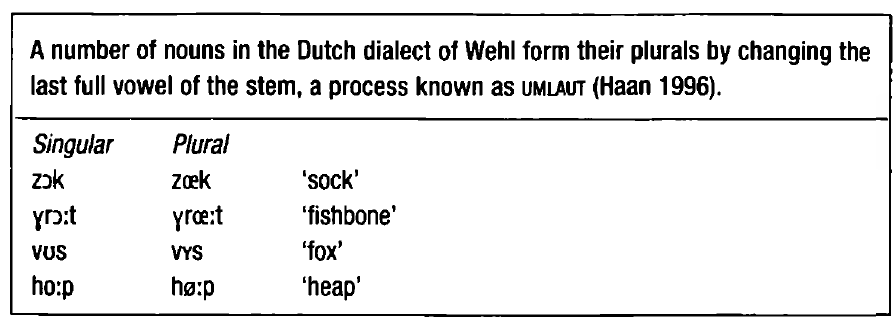
\includegraphics{../images/dutch.png}
\end{figure}

~\\
INSTRUCTOR NOTES: we look to see which vowels are affected, and compare them to see which feature is DIFFERENT (not e.g. what features they share); so since the vowels in the singular and plural are identical except that the singular forms are back and the plural are front, it's the feature [back] that is relevant / changing / involved (not e.g. the feature [round] just because all of the vowels are round)


\vfill
Excellent (3) ~~~ Good (2.2) ~~~ Fair (1.7) ~~~ Poor (0)
\newpage

\begin{center}
\textbf{{\color{red}{\HUGE END OF EXAM}}}\\

\end{center}
\newpage

\begin{center}
\textbf{{\color{blue}{\HUGE START OF EXAM\\}}}

\textbf{{\color{blue}{\HUGE Student ID: empty\\}}}

\textbf{{\color{blue}{\HUGE 4:30\\}}}

\end{center}
\newpage

\begin{center}
\textbf{{\color{blue}{\HUGE START OF EXAM\\}}}

\textbf{{\color{blue}{\HUGE Student ID: empty\\}}}

\textbf{{\color{blue}{\HUGE 4:40\\}}}

\end{center}
\newpage

\begin{center}
\textbf{{\color{blue}{\HUGE START OF EXAM\\}}}

\textbf{{\color{blue}{\HUGE Student ID: empty\\}}}

\textbf{{\color{blue}{\HUGE 4:50\\}}}

\end{center}
\newpage

\end{document}

